%\documentclass[handout]{beamer}
\documentclass[usenames,dvipsnames]{beamer}
\usepackage{amsmath}
\usepackage{stdpresent}
%\usepackage[margin=1in]{geometry}
\usepackage{tikz}
\usepackage{booktabs}
\usepackage{subcaption}
\usepackage{tikz}
\usetikzlibrary{intersections,positioning}
\usetikzlibrary{matrix, calc}
\newcommand*{\hnode}[1]{\node[outer sep=0pt,anchor=base] (#1) {#1};} 
\usepackage[absolute,overlay]{textpos}
\usetikzlibrary{bayesnet}
\usepackage{tcolorbox}
\usepackage[tikz]{bclogo}
\usepackage{textcomp}
\usepackage{vimacros}
\usepackage{physics}
\usepackage[round]{natbib}


\newcommand\Wider[2][3em]{%
\makebox[\linewidth][c]{%
  \begin{minipage}{\dimexpr\textwidth+#1\relax}
  \raggedright#2
  \end{minipage}%
  }%
}


\beamertemplatenavigationsymbolsempty
%\hypersetup{breaklinks=true, colorlinks=true, linkcolor=blue, citecolor=blue, urlcolor=blue}
\newcommand{\ack}[1]{\let\thefootnote\relax\footnote{\textcolor{gray}{#1}}}

\usepackage{tikz}
\usetikzlibrary{bayesnet}

\newcommand{\SDEC}{SDEC}
\newcommand{\SENT}{SENT}


%\DeclareMathOperator*{\softmax}{softmax}

\title[Word representation]{Deep latent models of word representation}


\def\W#1#2{\rnode{#1}{#2}\hfill}

\newcommand{\pointthis}[2]{
        \tikz[remember picture,baseline]{\node[anchor=base,inner sep=0,outer sep=0]%
        (#1) {\textbf{#1}};\node[overlay,rectangle callout,%
        callout relative pointer={(0.1cm,0.5cm)},fill=yellow!90] at ($(#1.north)+(-.5cm,-1cm)$) {#2};}%
        }%

\presetkeys{bclogo}{
ombre=true,
epBord=3,
couleur = blue!15!white,
couleurBord = red,
arrondi = 0.2,
logo=\bctrombone
}{}

\author[Wilker Aziz]{Wilker Aziz\\University of Amsterdam}
\date{April 3, 2018}

% add page num
\expandafter\def\expandafter\insertshorttitle\expandafter{%
  \insertshorttitle\hfill%
  \insertframenumber}

\begin{document}
\maketitlepage


\setcounter{framenumber}{0}




\frame[plain]{
	\frametitle{Word representation}
	
	\begin{textblock*}{\textwidth}(0.1\textwidth,0.2\textheight)
	
	An abstraction that stands for the use of a word
	
	~
	
	\only<1>{
	\begin{center}
	\textcolor{blue}{\emph{In the event of a chemical spill, most children know they should evacuate as advised by people in charge.}}
	\end{center}
	}
	\only<2->{
	\begin{center}
	\emph{\textcolor{blue}{In the event of a chemical spill, most children know they should} {\bf evacuate} \textcolor{blue}{as advised by people in charge.}}
	\end{center}	
	}
	\end{textblock*}
	
	%\begin{textblock*}{\textwidth}(0.1\textwidth,0.45\textheight)
	%\includegraphics<3>[scale=0.6]{img/repr/axes}
	%\includegraphics<4->[scale=0.6]{img/repr/axes-leave}
	%\end{textblock*}
	
	\begin{textblock*}{\textwidth}(0.4\textwidth,0.5\textheight)	
	\includegraphics<2->[scale=0.55]{img/repr/r2}	
	\end{textblock*}
	
	\begin{textblock*}{\textwidth}(0.1\textwidth,0.9\textheight)
	\only<3->{\alert{How do we choose the components?}}
	\end{textblock*}

}

\frame{
	\frametitle{Distributional Hypothesis}
	
	
	%\begin{textblock*}{\textwidth}(0.1\textwidth,0.2\textheight)
	\textcolor{blue}{Context} can represent the intended use of a word
	
	\begin{small}
	\only<1->{
	\begin{center}
	\emph{\textcolor{blue}{In the event of a chemical spill, most children know they should} \textcolor{black}{\bf evacuate} \textcolor{blue}{as advised by people in charge.}}
	\end{center}	
	}
	%\only<2->{
	%\begin{center}
	%\emph{\textcolor{blue}{In the event of a chemical spill, most children know they should} \arrowthis{evacuate}{ambiguity} \textcolor{blue}{as advised by people in charge.}}
	%\end{center}	
	%}
	\end{small}
	%\end{textblock*}
		
	%\begin{textblock*}{\textwidth}(0.1\textwidth,0.5\textheight)
	\begin{itemize}
		\item<1-> success hinges on {\bf discriminative power} of \textcolor{blue}{available context}
		%\item<2-> not limited to text
		%\begin{itemize}
		%	\item humans have access to rich sensorial context
		%\end{itemize}
		%\item<2-> but often \alert{crudely approximated} by text alone 
	\end{itemize}
	

	%\end{textblock*}
	
}
\frame[plain]{
	\frametitle{Discriminative embedding models}
	

	\begin{textblock*}{\textwidth}(0.1\textwidth,0.1\textheight)
	\begin{small}
	\begin{center}
	\only<1>{
	\emph{\textcolor{blue}{In the event of a chemical spill,} \textcolor{blue}{most children know they should} {\bf evacuate} \textcolor{blue}{as advised by people in} \textcolor{blue}{charge.}}}
	\only<2-4>{
	\emph{\textcolor{red}{In the event of a chemical spill,} \textcolor{blue}{most children know they should} {\bf evacuate} \textcolor{blue}{as advised by people in} \textcolor{red}{charge.}}}
	\only<5->{
	\emph{\textcolor{red}{In the event of a chemical spill,} \textcolor{blue}{most children know they should} \pointthis{evacuate}{ambiguity} \textcolor{blue}{as advised by people in} \textcolor{red}{charge.}}}
	\end{center}
	\end{small}
	\end{textblock*}
	
	
	\begin{textblock*}{\textwidth}(0.1\textwidth,0.37\textheight)
	
	\only<1->{
	Place words in $\mathbb R^d$ as to answer questions like

	\begin{center}	
	\emph{``Have I seen this word in this context?''}
	\end{center}
	}
	
	\only<2->{
	Fit a binary classifier \hfill \textcolor{gray}{\citep{goldberg2014word2vec}}
	\begin{itemize}
		\item \textcolor{blue}{positive} examples
		\item \alert{negative} examples\\ 		
	\end{itemize}
	}
	
	~
	
	\only<3->{
	``Far away'' context expresses a form of \alert{negative} correlation
	\begin{itemize}
		\item <4-> But data only show \textcolor{blue}{positive} examples
	\end{itemize}
	}
	
	\end{textblock*}
	

}


\frame{
	\frametitle{Limitations}
	
	Meaning representation is an {\bf unsupervised} problem
	\begin{itemize}
		\item we cannot actually observe what we are trying to learn \\
		i.e. representations
	\end{itemize}
	
	~
	
	\pause
	
	Distributional hypothesis seems pretty strong	
	\begin{itemize}
		\item but it fails when context is not sufficiently discriminative
	\end{itemize}
	

}


\frame{
	\frametitle{\textsc{EmbedAlign}}
	
	Generative treatment 
	\begin{itemize}
		\item model what we want to induce (i.e. representations)
		\item learn from \textcolor{blue}{{\bf positive examples}}
		\item learn from richer (less ambiguous) context
	\end{itemize}
	
	\ack{\citet{rios2018deep}}
	
}


\section{Embed-Align}

\frame[plain]{
	\frametitle{Equivalence through translation}
\Wider[4em]{

	\begin{textblock*}{\textwidth}(0.075\textwidth,0.2\textheight)
	\begin{tabular}{p{5cm} p{5cm}}
	\only<1->{
	\textcolor{blue}{In the event of a chemical spill, most children know they should {\bf evacuate} as advised by people in charge.
	}
	} & 
	\only<2->{
	\textcolor{orange!90!yellow}{Em caso de vazamento qu\'imico, a maioria das crian\c{c}as est\~{a}o conscientes de que devem  {\bf deixar} o local, como sugerem autoridades.}
	} \\
	 & \\
	\only<1->{	
	\textcolor{blue}{After ingestion, the substance speeds up the movement of your bowels encouraging you to {\bf evacuate}.}} &
	\only<2->{
	\textcolor{orange!90!yellow}{Ap\'os ingerida, a subst\^ancia acelera o movimento das paredes do intestino for\c{c}ando o indiv\'iduo a se {\bf aliviar}.}
	}	
	\end{tabular}
	\end{textblock*}
	
}

	\only<3>{
	\begin{textblock*}{\textwidth}(0.075\textwidth,0.8\textheight)
	Observation from WSD community
	\begin{itemize}
		\item foreign text as {\bf proxy to sense supervision} \\
		\textcolor{gray}{(Diab and Resnik, 2002)}
	\end{itemize}
	\end{textblock*}
	}
	
}


\frame[plain]{
	\frametitle{Embed-Align}
	
	\begin{textblock*}{\textwidth}(0.1\textwidth,0.1\textheight)
	\begin{center}
		\textcolor{blue}{quickly evacuate the area} ~ / ~  \textcolor{orange!90!yellow}{deixe o local rapidamente}
	\end{center}
	\end{textblock*}
	
	\only<7->{
	\begin{textblock*}{0.3\textwidth}(0.025\textwidth,0.3\textheight)
	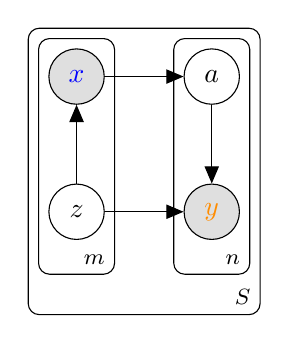
\begin{tikzpicture}
    % Define nodes
    \node[obs]						(y)		{\textcolor{orange!90!yellow}{$ y $}};
    \node[latent, above = of y]		(a)		{$ a $};
    \node[obs, left = of a]		(x)		{\textcolor{blue}{$ x $}};
    \node[latent, below = of x]		(z)		{$ z $};
    
    % Connect nodes
    \edge{a}{y};
    \edge{x}{a};
    \edge{z}{x, y};
    
    % add plates
    \plate {x-sentence} {(x)(z)} {$ m $};
    \plate {y-sentence} {(y)(a)} {$ n $};
    \plate {corpus} {(y-sentence)(x-sentence)} {$ S $};
    \end{tikzpicture}
	\end{textblock*}
	}
	
	\begin{textblock*}{\textwidth}(0.32\textwidth,0.3\textheight)
	

	\begin{small}
			\begin{tabular}{p{0.5cm} | p{1.5cm} p{1.5cm} p{1.5cm} p{1.5cm}}
			\only<3->{$X$ & \textcolor{blue}{quickly$_1$} & \textcolor{blue}{evacuate$_2$} & \textcolor{blue}{the$_3$} & \textcolor{blue}{area$_4$}}\\
			\only<3->{& $\uparrow$ & $\uparrow$ & $\uparrow$ & $\uparrow$ }\\
			\only<2->{$Z$ & $z_{\textcolor{blue}{1}}$ & $z_{\textcolor{blue}{2}}$ & $z_{\textcolor{blue}{3}}$ & $z_{\textcolor{blue}{4}}$} \\
			& & & & \\
			\only<4->{$A$ & $a_{\textcolor{orange!90!yellow}{1}}=\textcolor{blue}{2}$ & $a_{\textcolor{orange!90!yellow}{2}}=\textcolor{blue}{3}$ & $a_{\textcolor{orange!90!yellow}{3}}=\textcolor{blue}{4}$ & $a_{\textcolor{orange!90!yellow}{4}}=\textcolor{blue}{1}$}\\
			\only<5->{$Z_a$ & $z_{\textcolor{blue}{2}}$ & $z_{\textcolor{blue}{3}}$ & $z_{\textcolor{blue}{4}}$ & $z_{\textcolor{blue}{1}}$} \\
			\only<6->{& $\downarrow$ & $\downarrow$ & $\downarrow$ & $\downarrow$}\\
			\only<6->{$Y$ & \textcolor{orange!90!yellow}{deixe$_1$} & \textcolor{orange!90!yellow}{o$_2$} & \textcolor{orange!90!yellow}{local$_3$} & \textcolor{orange!90!yellow}{rapidamente$_4$}} \\
			\end{tabular}
	\end{small}
	\end{textblock*}
	
	\begin{textblock*}{\textwidth}(0.1\textwidth,0.8\textheight)
	\only<7>{Marginalising alignments collects additional training data for $z$}
	\end{textblock*}

}


\frame[plain]{
	\frametitle{How does it disambiguate?}
	
	\begin{textblock*}{0.45\textwidth}(0.01\textwidth,0.1\textheight)	
	\only<2>{
	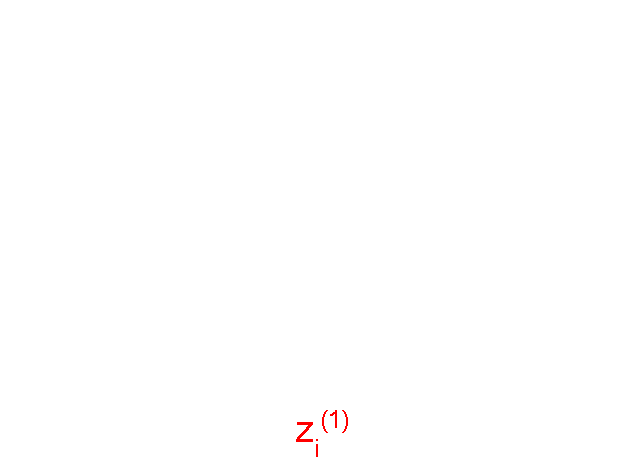
\includegraphics[scale=0.6]{img/cmp/z1}
	}
	\only<3-7>{
	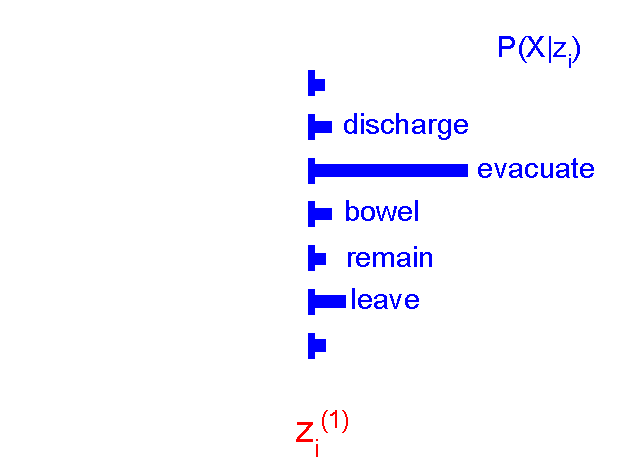
\includegraphics[scale=0.6]{img/cmp/x1}
	}
	\only<8->{
	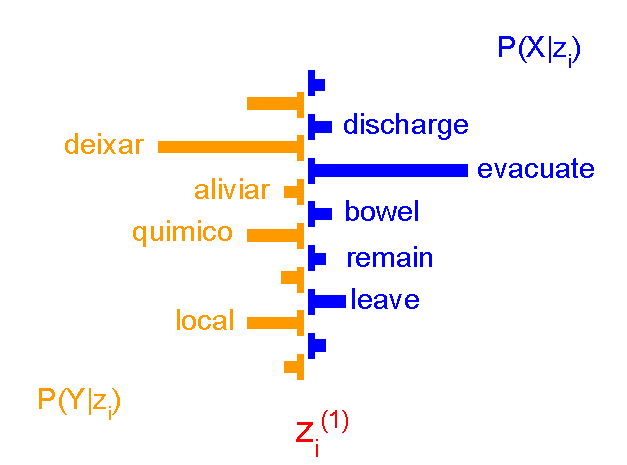
\includegraphics[scale=0.6]{img/cmp/y1}
	}
	\end{textblock*}
	
	\begin{textblock*}{0.5\textwidth}(0.55\textwidth,0.1\textheight)	
	\only<5>{
	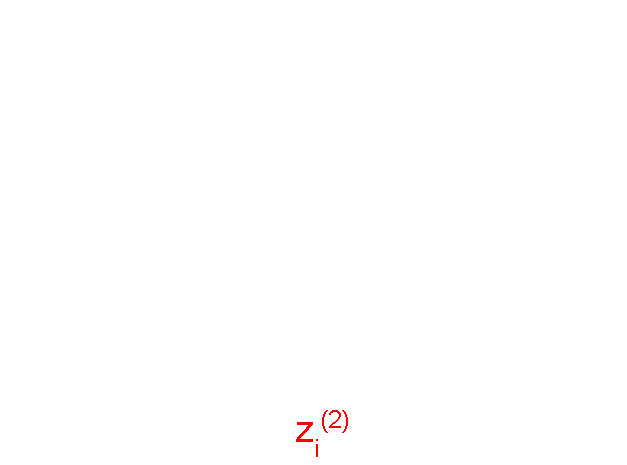
\includegraphics[scale=0.6]{img/cmp/z2}
	}
	\only<6-7>{
	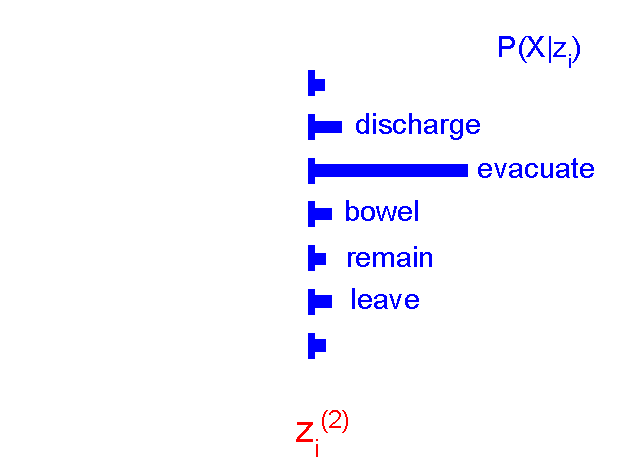
\includegraphics[scale=0.6]{img/cmp/x2}
	}
	\only<8->{
	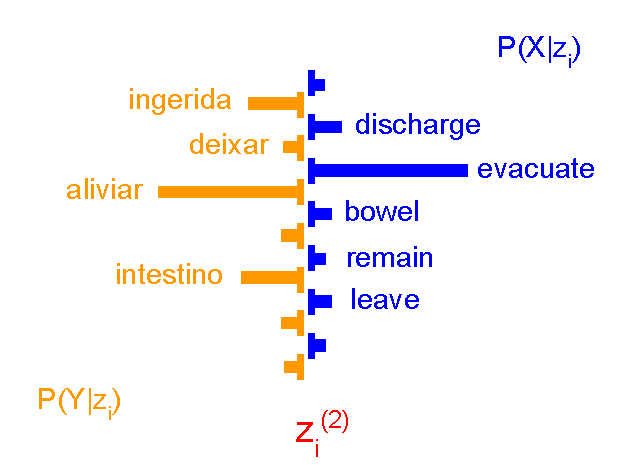
\includegraphics[scale=0.6]{img/cmp/y2}
	}
	\end{textblock*}
	
	
	\begin{textblock*}{0.5\textwidth}(0.05\textwidth,0.7\textheight)	
	\begin{footnotesize}
	\begin{tabular}{p{5.2cm} | p{5.2cm}}
	
	\textcolor{blue}{In the event of a chemical spill, most children know they should {\bf evacuate}$_i$ as advised by people in charge.}
	&  
	\only<4->{\textcolor{blue}{After ingestion, the substance  speeds up the movement of your bowels encouraging you to {\bf evacuate}$_i$.}}
	\\
	& \\
	\only<7->{\textcolor{orange!90!yellow}{Em caso de vazamento qu\'imico, a maioria das crian\c{c}as est\~{a}o conscientes de que devem  {\bf deixar} o local, como sugerem autoridades.}}
	& 
	\only<7->{
	\textcolor{orange!90!yellow}{Ap\'os ingerida, a subst\^ancia acelera o movimento das paredes do intestino for\c{c}ando o indiv\'iduo a se {\bf aliviar}.}
	}
	\end{tabular}
	\end{footnotesize}
	\end{textblock*}
	
}


\frame[plain]{
	\frametitle{Tractable inference}

		\begin{textblock*}{0.35\textwidth}(0.8\textwidth,0.05\textheight)
		\begin{center}
		\only<1>{\includegraphics<1>[scale=0.7]{img/bidir}\\}
		\only<2->{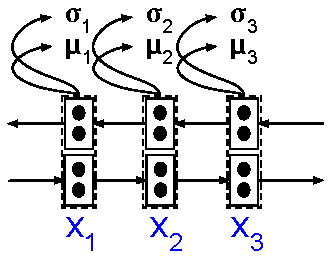
\includegraphics[scale=0.7]{img/meanstd}\\}		
		\hfill\textcolor{blue}{Evacuate$_1$ the$_2$ area$_3$}
		\end{center}
		\end{textblock*}


	\begin{textblock*}{\textwidth}(0.05\textwidth,0.15\textheight)
	\begin{enumerate} \small
		\item<1-> Read sentence
		\item<2-> Predict posterior mean $\mu_i$ and std $\sigma_i$
		%\begin{columns}
		%\begin{column}{0.4\textwidth}
		%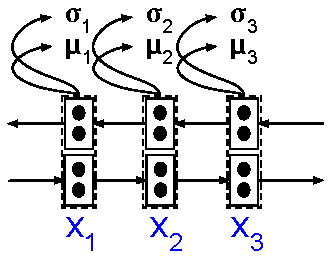
\includegraphics[scale=0.4]{img/meanstd}
		%\end{column}
		%\begin{column}{0.4\textwidth}
		%\hfill\textcolor{blue}{Evacuate$_1$ the$_2$ area$_3$}
		%\end{column}
		%\end{columns}
		\item<3-> Sample $Z_i \sim \mathcal N(\mu_i, \sigma^2_i)$
		%$z_i = \mu_i + \sigma_i \epsilon_i$ \\
		%where $\epsilon_i \sim \mathcal N(0,I)$ 
		\item<4-> Predict categorical distributions
		\item<5-> Generate observations \\ %by marginalising latent alignments\\
		\textcolor{blue}{Evacuate$_1$ the$_2$ area$_3$} ~/~ \textcolor{orange!90!yellow}{Deixe$_1$ o$_2$ local$_3$} \\
		
		%\begin{itemize}
		%	\item $P_\theta(x_1^m|z_1^m) = \prod_{i=1}^m P_\theta(X=x_i|z_i)$
		%	\item $P_\theta(y_1^m|x_1^m, z_1^m) = \prod_{j=1}^n \sum_{a_j=1}^m P(a_j|m) P_\theta(Y=y_j|z_i)$
		%\end{itemize}
		\item<6-> Maximise a lowerbound on likelihood\\
		\textcolor{gray}{(Kingma and Welling, 2014)}
	\end{enumerate}		
	\end{textblock*}
	
	\begin{textblock*}{\textwidth}(0.05\textwidth,0.7\textheight)
	\only<2>{		
	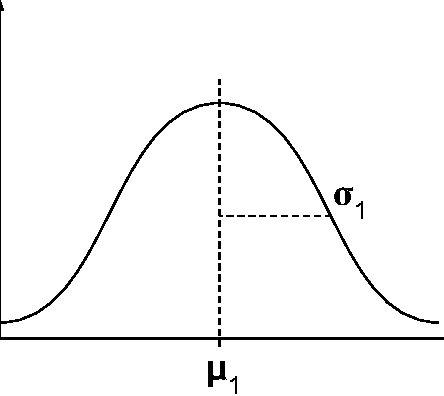
\includegraphics[scale=0.5]{img/N1}~
	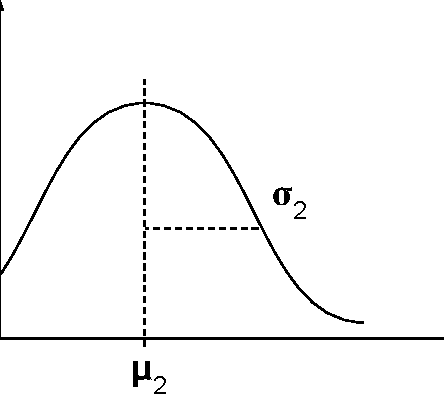
\includegraphics[scale=0.5]{img/N2}~
	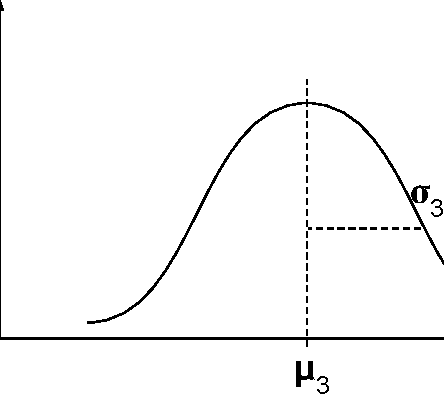
\includegraphics[scale=0.5]{img/N3}
	}
	\only<3>{
	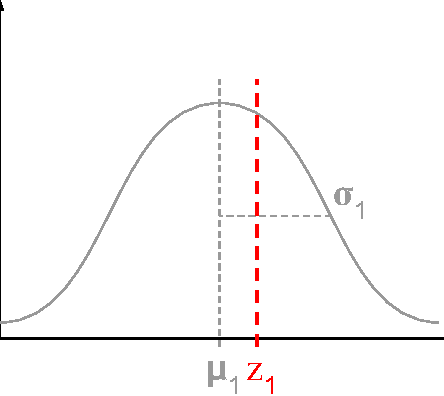
\includegraphics[scale=0.5]{img/Z1}~
	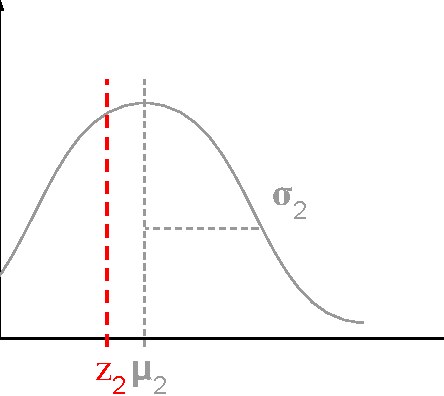
\includegraphics[scale=0.5]{img/Z2}~
	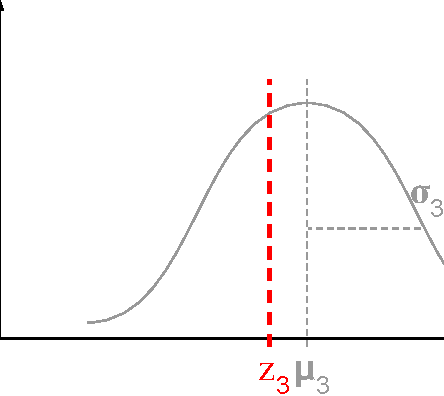
\includegraphics[scale=0.5]{img/Z3}
	}
	\only<4->{
	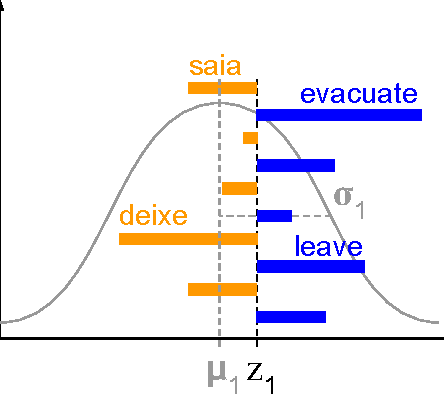
\includegraphics[scale=0.5]{img/P1}~
	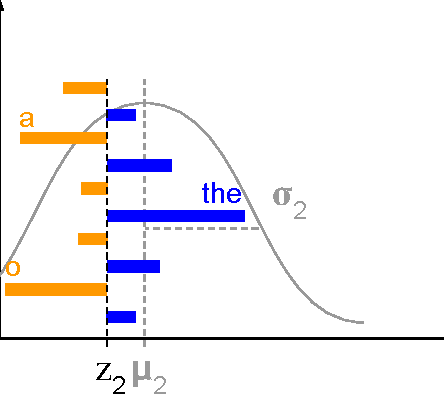
\includegraphics[scale=0.5]{img/P2}~
	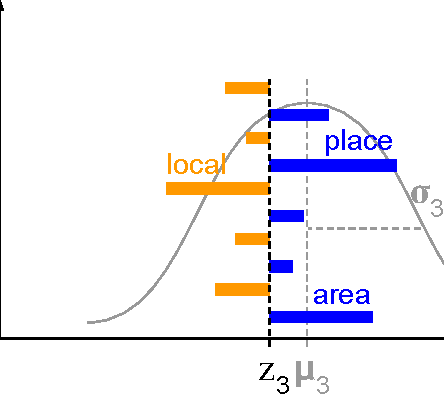
\includegraphics[scale=0.5]{img/P3}
	}
	\end{textblock*}
	
}

\frame[plain]{
	\frametitle{What's special about it?}
	
	\begin{textblock*}{0.75\textwidth}(0.05\textwidth,0.2\textheight)
	The model reads English text and 
	\begin{itemize}
		\item<2-> \alert{predicts uncertainty}
		\item<2-> \textcolor{orange!90!yellow}{describes ``sense'' using Portuguese words}
	\end{itemize}
	\end{textblock*}
	
	\begin{textblock*}{0.35\textwidth}(0.8\textwidth,0.05\textheight)
		\begin{center}
		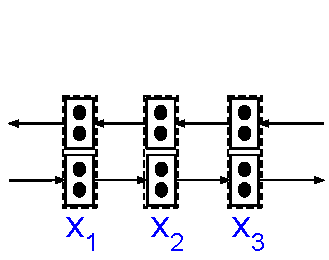
\includegraphics[scale=0.7]{img/bidir}\\		
		\hfill\textcolor{blue}{Evacuate$_1$ the$_2$ area$_3$}
		\end{center}
	\end{textblock*}
	
	\only<2->{
	\begin{textblock*}{0.5\textwidth}(0.1\textwidth,0.4\textheight)
		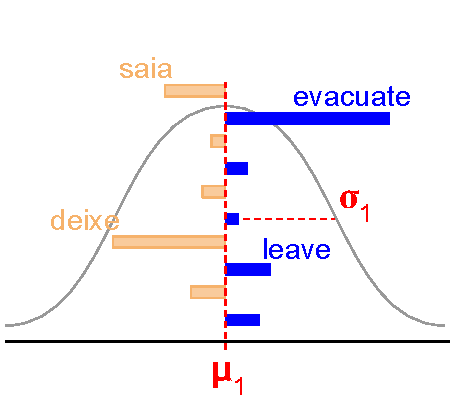
\includegraphics[scale=0.7]{img/sense1/mean}\\		
	\end{textblock*}
	}

}


\begin{frame}[plain]{Complete specification}
Generative model: for $i=1, \ldots, m$ and $j=1, \ldots, n$ \pause
\begin{equation*}
\begin{aligned}
Z_i &\sim \mathcal N(0, I) \\ \pause
X_i|z_i &\sim \Cat(\mathbf f_i) \\ 
\mathbf f_i &= \softmax(\affine_\theta(z_i)) \\ \pause
A_j|m &\sim \mathcal U(1/m) \\ \pause
Y_j|z_1^m, a_j &\sim \Cat(\mathbf g_{a_j}) \\
\mathbf g_{a_j} &= \softmax(\affine_\theta(z_{a_j}))
\end{aligned}
\end{equation*}

Inference model: for $i=1, \ldots, m$ \pause
\begin{equation*}
\begin{aligned}
Z_i|x_1^m &\sim \mathcal N(\mathbf u_i, \diag(\mathbf s_i \odot \mathbf s_i))\\ \pause
\mathbf h_1^m &= \text{enc}_\lambda(x_1^m) \\ \pause
\mathbf u_i &= \text{affine}_\lambda(\relu(\text{affine}_\lambda(\mathbf h_i)))\\ \pause
\mathbf s_i &= \softplus_\lambda(\relu(\text{affine}_\lambda(\mathbf h_i))) 
\end{aligned}
\end{equation*}

\ack{\citet{rios2018deep}}
\end{frame}

\begin{frame}{ELBO}

ELBO
\begin{equation*}
\begin{aligned}
\mathbb E_{q_\lambda(z_1^m|x_1^m)}\left[ \log P_\theta(x_1^m, y_1^n|z_1^m)\right] - \textcolor{blue}{\KL{q_\lambda(z_1^m|x_1^m)}{p(z_1^m)} }
\end{aligned}
\end{equation*}

\pause

KL term
\begin{small}
\begin{equation*}
\begin{aligned}
\textcolor{blue}{\KL{q_\lambda(z_1^m|x_1^m)}{p(z)} }
&= \underbrace{\sum_{i=1}^m \KL{q_\lambda(z_i|x_1^m)}{p(z_1^m)}}_{\text{mean field}} \\ \pause
&= \sum_{i=1}^m \KL{\underbrace{\mathcal N(\mathbf u_i, \diag(\mathbf s_i \odot \mathbf s_i))}_{\text{inference model}}}{\underbrace{\mathcal N(0, I)}_{\text{prior}}} \
\end{aligned}
\end{equation*}
\end{small}


\end{frame}

\begin{frame}{ELBO - L1 term}

ELBO
\begin{equation*}
\begin{aligned}
\textcolor{blue}{\mathbb E_{q_\lambda(z_1^m|x_1^m)}\left[ \log P_\theta(x_1^m, y_1^n|z_1^m)\right]} - \KL{q_\lambda(z_1^m|x_1^m)}{p(z_1^m)} 
\end{aligned}
\end{equation*}

\pause

Likelihood term
\begin{small}
\begin{equation*}
\begin{aligned}
&\textcolor{blue}{\mathbb E_{q_\lambda(z_1^m|x_1^m)}\left[ \log P_\theta(x_1^m, y_1^n|z_1^m)\right]} \\ \pause
&= \underbrace{\textcolor{purple}{\mathbb E_{q_\lambda(z_1^m|x_1^m)}\left[ \log P_\theta(x_1^m|z_1^m)\right]} + \mathbb E_{q_\lambda(z_1^m|x_1^m)}\left[ \log P_\theta(y_1^n|m, z_1^m)\right]}_{\text{conditional independence}}
\end{aligned}
\end{equation*}
\end{small}

\pause
L1 term
\begin{small}
\begin{equation*}
\begin{aligned}
\textcolor{purple}{\mathbb E_{q_\lambda(z_1^m|x_1^m)}\left[ \log P_\theta(x_1^m|z_1^m)\right]} 
&= \sum_{i=1}^m \mathbb E_{q_\lambda(z_i|x_1^m)}\left[ \log P_\theta(x_i|z_i)\right] \\ \pause
&= \sum_{i=1}^m \mathbb E_{q_\lambda(z_i|x_1^m)} \left[ \log \Cat(x_i|\mathbf f_i)\right] 
\end{aligned}
\end{equation*}
\end{small}


\end{frame}



\begin{frame}[plain]{ELBO - L2 term}

L2 term
\begin{small}
\begin{equation*}
\begin{aligned}
\mathbb E_{q_\lambda(z_1^m|x_1^m)}\left[ \log P_\theta(y_1^n|m, z_1^m)\right] 
\pause &= \mathbb E_{q_\lambda(z_1^m|x_1^m)}\left[ \log \prod_{j=1}^n P_\theta(y_j|m, z_1^m)\right]  \\ \pause
&= \mathbb E_{q_\lambda(z_1^m|x_1^m)}\left[  \sum_{j=1}^n \log P_\theta(y_j|m, z_1^m)\right]   \\ \pause
&= \mathbb E_{q_\lambda(z_1^m|x_1^m)}\left[  \sum_{j=1}^n \log \sum_{a_j}^m P_\theta(y_j, a_j|m, z_1^m)\right]   \\ \pause
&= \mathbb E_{q_\lambda(z_1^m|x_1^m)}\left[  \sum_{j=1}^n \log \sum_{a_j}^m P(a_j|m) P_\theta(y_j|z_{a_j}) \right]  \\  \pause
%&\overset{\text{JI}}{\ge} \mathbb E_{q_\lambda(z_1^m|x_1^m)}\left[  \sum_{j=1}^n \mathbb E_{\mathcal U(A_j|m)} [\log P_\theta(y_j|z_{A_j}) ]\right]  \\  
&= \mathbb E_{q_\lambda(z_1^m|x_1^m)}\left[  \sum_{j=1}^n \log \sum_{a_j}^m \mathcal U(a_j|1/m) \Cat(y_j|\mathbf g_{a_j})\right]
\end{aligned}
\end{equation*}
\end{small}


\end{frame}

\begin{frame}[plain]{ELBO - Lowerbound on L2 term}

L2 term
\begin{small}
\begin{equation*}
\begin{aligned}
\mathbb E_{q_\lambda(z_1^m|x_1^m)}\left[ \log P_\theta(y_1^n|m, z_1^m)\right] 
 &= \mathbb E_{q_\lambda(z_1^m|x_1^m)}\left[  \sum_{j=1}^n \log \sum_{a_j}^m P(a_j|m) P_\theta(y_j|z_{a_j}) \right]  \\  \pause
 &= \mathbb E_{q_\lambda(z_1^m|x_1^m)}\left[  \sum_{j=1}^n \log \mathbb E_{P(a_j|m)} \left[ P_\theta(y_j|z_{a_j}) \right] \right]  \\  \pause
&\overset{\text{JI}}{\ge} \mathbb E_{q_\lambda(z_1^m|x_1^m)}\left[  \sum_{j=1}^n \mathbb E_{P(a_j|m)} [\log P_\theta(y_j|z_{a_j}) ]\right]  \\  \pause
&= \mathbb E_{q_\lambda(z_1^m|x_1^m)}\left[  \sum_{j=1}^n \mathbb E_{\mathcal U(a_j|m)} [\log \Cat(y_j|\mathbf g_{a_j}) ]\right] 
\end{aligned}
\end{equation*}
\end{small}

\pause

Alignment model $P(a_j|m)=\frac{1}{m}$ is not a function of $\theta$
\begin{itemize}
	\item we can make an MC estimate by sampling candidate alignments uniformly
\end{itemize}

\ack{You may skip over this slide.}

\end{frame}

\begin{frame}{The softmax problem}
Categorical parameters are expensive to compute 
\begin{equation*}
\begin{aligned}
X &\sim \Cat(\mathbf f)\\
\mathbf f &= \softmax (\hat{\mathbf f}) \\
f_{x} &= \frac{\exp(\hat f_x)}{\sum_{x' \in \mathcal X} \exp(\hat f_{x'})}
\end{aligned}
\end{equation*}

\pause

\begin{itemize}
	\item $\mathbf f_1^m$ requires normalising $m$ distributions over the vocabulary of L$_1$, thus it takes time $O(m \times v_1)$
	\item $\mathbf g_1^m$ requires normalising $m$ distributions over the vocabulary of L$_2$, thus it takes time $O(m \times v_2)$
\end{itemize}

\ack{$v_1 = |\mathcal X|$ is the size of the vocabulary of $L_1$; $v_2 = |\mathcal Y|$ is the size of the vocabulary of $L_2$}

\end{frame}

\begin{frame}{Efficient softmax}
Logistic regression
\begin{equation*}
P(X=x|z) = \frac{\exp(s(z, x))}{\sum_{x'\in \mathcal X} \exp(s(z, x'))}
\end{equation*}

\pause

Define
\begin{itemize}
	\item a set $\mathcal C(x)$ such that $x \in \mathcal C$
	\item a set $\mathcal N(x)$ such that $\mathcal C(x) \cap \mathcal N(x) = \emptyset$
\end{itemize}

\pause 
Re-express normaliser for $P(X=x|z)$ 
\begin{equation*}
\sum_{x'\in \mathcal X} \exp(s(z, x')) = \sum_{x'\in \mathcal C(x)} \exp(s(z, x')) + \sum_{x'\in \mathcal N(x)} \kappa(x')\exp(s(z, x'))
\end{equation*}
\begin{itemize}
	\item $\kappa(x') = \frac{1}{q(x')}$ and $q(x')$ is an importance distribution
\end{itemize}

\end{frame}

\begin{frame}{Approximate $P_{X|Z}$}

Logistic regression
\begin{equation*}
P_\theta(x|z) = \frac{\exp(s_\theta(z, x))}{\sum_{x'\in \mathcal X} \exp(s_\theta(z, x'))}
\end{equation*}

\pause

Build
\begin{itemize}
	\item a set $\mathcal C$ containing all L$_1$ words in batch
	\item a set $\mathcal N$ sampling uniformly without replacement from $\mathcal X \setminus \mathcal C$
\end{itemize}

\pause 
Approximate normaliser for $P_\theta(x|z)$
\begin{equation*}
\sum_{x'\in \mathcal X} \exp(s_\theta(z, x')) \approx \sum_{x'\in \mathcal C} \exp(s_\theta(z, x')) + \sum_{x'\in \mathcal N} \frac{|\mathcal X \setminus \mathcal C|}{|\mathcal N|}\exp(s_\theta(z, x'))
\end{equation*}
\begin{itemize}
	\item $s_\theta(z, x) = z^\top \mathbf c_x + b_x$ \\
	$\mathbf c_x = \text{lookup}_\theta(x)$ is a deterministic embedding, $b_x$ a bias term
\end{itemize}

\end{frame}

\begin{frame}{Approximate $P_{Y|Z}$}

Logistic regression
\begin{equation*}
P_\theta(y|z) = \frac{\exp(u_\theta(z, y))}{\sum_{y'\in \mathcal Y} \exp(u_\theta(z, y'))}
\end{equation*}

\pause

Build
\begin{itemize}
	\item a set $\mathcal C$ containing all L$_2$ words in batch
	\item a set $\mathcal N$ sampling uniformly without replacement from $\mathcal Y \setminus \mathcal C$
\end{itemize}

\pause 
Approximate normaliser for $P_\theta(y|z)$
\begin{equation*}
\sum_{y'\in \mathcal X} \exp(s_\theta(z, y')) \approx \sum_{y'\in \mathcal C} \exp(s_\theta(z, y')) + \sum_{y'\in \mathcal N} \frac{|\mathcal Y \setminus \mathcal C|}{|\mathcal N|}\exp(s_\theta(z, y'))
\end{equation*}
\begin{itemize}
	\item $s_\theta(z, y) = z^\top \mathbf c_y + b_y$ \\
	$\mathbf c_y = \text{lookup}_\theta(y)$ is a deterministic embedding, $b_y$ a bias term
\end{itemize}

\end{frame}

\begin{frame}{Complementary Sum Sampling (CSS) - Summary}
The approximation effectively reduces the size of the support of the categorical variable
\begin{itemize}
	\item in each batch, the support is made of the word types in the batch
	\item along with a random subset of ``negative words''
	\item this is similar to ``negative sampling'' but improves on asymptotic behaviour
	\item it only affects the softmax: the model remains generative
\end{itemize}

\ack{\citet{botev2017complementary}}
\end{frame}




\section{Bayesian Skip-Gram}

\begin{frame}[plain]{Bayesian Skip-Gram}


\begin{columns}
\begin{column}{0.45\textwidth}
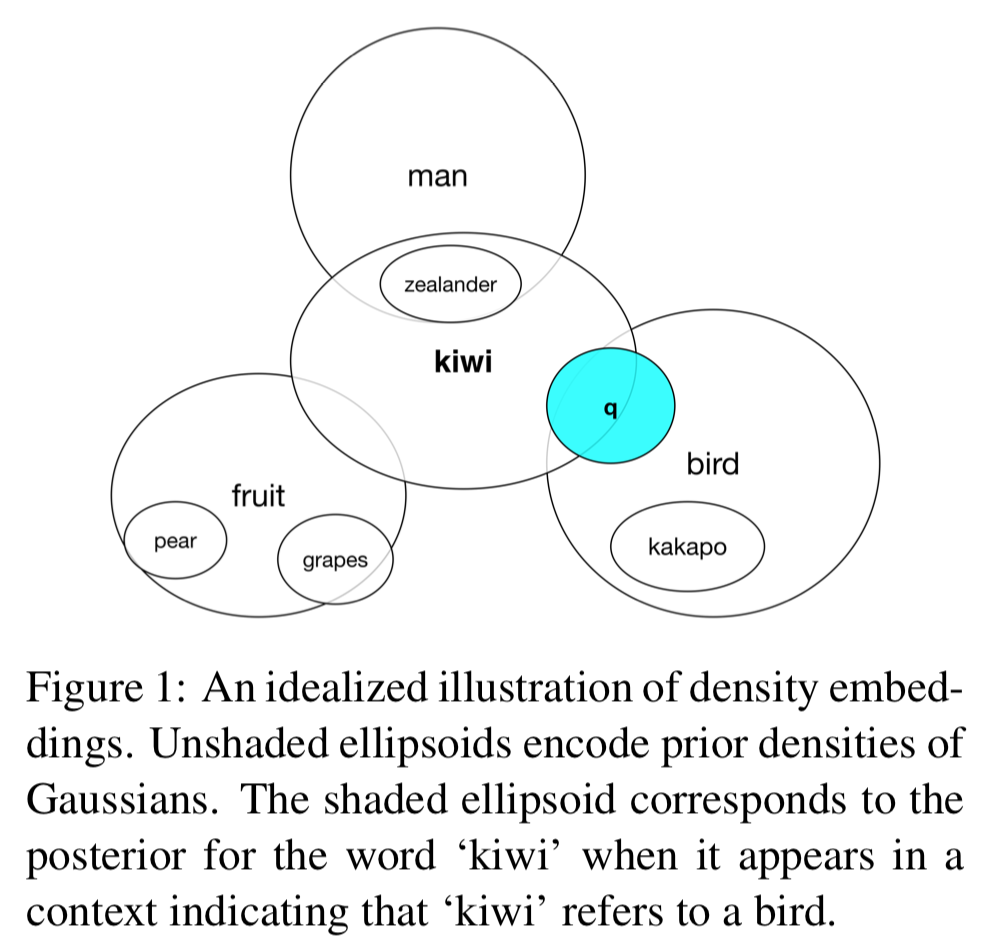
\includegraphics[scale=0.35]{img/bsg-example}
\end{column}
\quad
\begin{column}{0.45\textwidth}
\begin{footnotesize}
\only<1>{
\emph{``Representing a word as a distribution provides many potential benefits. For example, such embeddings let us encode generality of terms (e.g., `kakapo' is a type of `bird'), characterize uncertainty about semantic properties of the corresponding referent (e.g., a proper noun, such as `John', encodes little about the person it refers to) or represent polysemy (e.g., `kiwi' may refer to a fruit, a bird or a New Zealander).''}
}
\only<2>{
\emph{``In principle, using densities to represent words provides a natural way of encoding entailment: the decision regarding entailment relation can be made by testing the level sets of the distributions for `soft inclusion'. For example, in Figure 1, the ellipse for `kakapo' lies within the ellipse for `bird'. ''}
}
\end{footnotesize}
\end{column}

\end{columns}


\ack{\citet{bravzinskas2017embedding}}
\end{frame}


\begin{frame}[plain]{Complete specification}
Generative model: for $i=1, \ldots, m$\\

\begin{equation*}
\begin{aligned}
Z_i|x_i &\sim \mathcal N(\boldsymbol \mu_{x_i}, \diag(\boldsymbol \sigma_{x_i} \odot \boldsymbol \sigma_{x_i}))\\
\boldsymbol \mu_{x_i} &= \text{lookup}_\theta(x_i)\\
\boldsymbol \sigma_{x_i} &= \softplus(\text{lookup}_\theta(x_i))
\end{aligned}
\end{equation*}
\pause
~for $k \in \mathcal K_i = \{\underbrace{i-n, \ldots, i-1,  i+1, \ldots, i+n}_{n \text{ words on each side of }x_i}\}$ \pause
\begin{equation*}
\begin{aligned}
X_k|z_i &\sim \Cat(\mathbf f_i) \\ 
\mathbf f_i &= \softmax(\affine_\theta(z_i))
\end{aligned}
\end{equation*}

\pause

Inference model
\begin{equation*}
\begin{aligned}
Z_i|x_{i-n}^{i+n} &\sim \mathcal N(\mathbf u_i, \diag(\mathbf s_i \odot \mathbf s_i))\\
\mathbf h_i &= \sum_{k \in \mathcal K_i} \relu(\affine_\lambda([x_k, x_i])) \\
\mathbf u_i &= \affine_\lambda(h_i) \\
\mathbf s_i &= \softplus(\affine_\lambda(h_i)) 
\end{aligned}
\end{equation*}


\end{frame}

\begin{frame}{ELBO}
\begin{equation*}
\begin{aligned}
\mathbb E_{q_\lambda(z_1^m|x_1^m)} \left[ \log \alert{\prod_{i=1}^m \prod_{k \in \mathcal K_i} P(x_k|z_i)} \right] - \KL{q_\lambda(z_1^m|x_1^m)}{p_\theta(z_1^m|x_1^m)}
\end{aligned}
\end{equation*}
\begin{itemize}
	\item observation model is trained discriminatively\\
	latent variables generate overlapping subsets of observations
\end{itemize}

\end{frame}

\begin{frame}{ELBO - KL term}
\begin{equation*}
\begin{aligned}
\mathbb E_{q_\lambda(z_1^m|x_1^m)} \left[ \log \prod_{i=1}^m \prod_{k \in \mathcal K_i} P_\theta(x_k|z_i) \right] - \textcolor{blue}{\KL{q_\lambda(z_1^m|x_1^m)}{p_\theta(z_1^m|x_1^m)}}
\end{aligned}
\end{equation*}

KL term
\begin{equation*}
\begin{aligned}
&\textcolor{blue}{\KL{q_\lambda(z_1^m|x_1^m)}{p_\theta(z_1^m|x_1^m)}} \\ \pause
 &=  \sum_{i=1}^m \KL{q_\lambda(z_i|x_{i-n}^{i+n})}{p_\theta(z_i|x_i)} \\ \pause
 &=  \sum_{i=1}^m \KL{\underbrace{\mathcal N(\mathbf u_i, \diag(\mathbf s_i \odot \mathbf s_i))}_{\text{inference model}}}{\underbrace{\mathcal N(\boldsymbol \mu_{x_i}, \diag(\boldsymbol \sigma_{x_i} \odot \boldsymbol \sigma_{x_i}))}_{\text{prior}}} 
\end{aligned}
\end{equation*}

\ack{Empirical Bayes: point estimate prior parameters}

\end{frame}


\begin{frame}{ELBO - Likelihood term}
\begin{equation*}
\begin{aligned}
\textcolor{blue}{\mathbb E_{q_\lambda(z_1^m|x_1^m)} \left[ \log \prod_{i=1}^m \prod_{k \in \mathcal K_i} P_\theta(x_k|z_i) \right]} - \KL{q_\lambda(z_1^m|x_1^m)}{p_\theta(z_1^m|x_1^m)}
\end{aligned}
\end{equation*}
\pause

Likelihood term
\begin{small}
\begin{equation*}
\begin{aligned}
\textcolor{blue}{\mathbb E_{q_\lambda(z_1^m|x_1^m)} \left[ \log \prod_{i=1}^m \prod_{k \in \mathcal K_i} P_\theta(x_k|z_i) \right]}  \pause
 &= \mathbb E_{q_\lambda(z_1^m|x_1^m)} \left[  \sum_{i=1}^m \sum_{k \in \mathcal K_i} \log P_\theta(x_k|z_i) \right] \\ \pause
&= \sum_{i=1}^m \sum_{k \in \mathcal K_i} \mathbb E_{q_\lambda(z_i|x_{i-n}^{i+n})} \left[  \log P_\theta(x_k|z_i) \right] \\ \pause
&= \sum_{i=1}^m \sum_{k \in \mathcal K_i} \mathbb E_{q_\lambda(z_i|x_{i-n}^{i+n})} \left[  \log \Cat(x_k|\mathbf f_i) \right]
\end{aligned}
\end{equation*}
\end{small}

\end{frame}

\begin{frame}{The softmax problem}

To circumvent an expensive softmax, change the likelihood term
\begin{equation*}
P_\theta(x|z) = \frac{u_\theta(z, x)}{\alert{\sum_{x' \in \mathcal X} u_\theta(z, x')}} \qquad \text{with } u_\theta(\cdot, \cdot) > 0
\end{equation*}
\pause
and re-write the likelihood term
\begin{equation*}
\begin{aligned}
\mathbb E_{q_\lambda(z)} \left[  \log P_\theta(x|z) \right] 
 &= \mathbb E_{q_\lambda(z)} \left[  \log u_\theta(z, x) - \log \alert{\sum_{x'\in \mathcal X}u_\theta(z, x')}\right] \\ \pause
 &=\mathbb E_{q_\lambda(z)} \left[  \log u_\theta(z, x) \right] - \mathbb E_{q_\lambda(z)} \left[ \log \alert{\sum_{x'\in \mathcal X}u_\theta(z, x')}\right]
\end{aligned}
\end{equation*}


\end{frame}

\begin{frame}[plain]{Lowerbound on likelihood term}
Then (by design) let
\begin{equation*}
u_\theta(z, x) = \underbrace{P(x)}_{\text{fixed}}\mathcal N(z|\boldsymbol \mu_x, \diag(\boldsymbol \sigma_x \odot \boldsymbol \sigma_x))
\end{equation*}
\pause

And bound $ \mathbb E_{q_\lambda(z)} \left[ \log \alert{\sum_{x'\in \mathcal X}u_\theta(z, x')}\right] $ \pause
\begin{equation*}
\begin{aligned} 
&=\mathbb E_{q_\lambda(z)} \left[ \log \alert{\sum_{x'\in \mathcal X} P(x)\mathcal N(z|\boldsymbol \mu_x, \diag(\boldsymbol \sigma_x \odot \boldsymbol \sigma_x))} \right] \\ \pause
&=\mathbb E_{q_\lambda(z)} \left[ \log \alert{\mathbb E_{P(x)}\left[ \mathcal N(z|\boldsymbol \mu_x, \diag(\boldsymbol \sigma_x \odot \boldsymbol \sigma_x)) \right]} \right] \\ \pause
&\overset{\text{JI}}{\ge} \mathbb E_{q_\lambda(z)} \left[ \textcolor{blue}{\mathbb E_{P(x)}\left[ \log \mathcal N(z|\boldsymbol \mu_x, \diag(\boldsymbol \sigma_x \odot \boldsymbol \sigma_x)) \right]} \right]
\end{aligned}
\end{equation*}
\pause

\begin{itemize}
	\item $P(x)$ does not depend on $\theta$, we can compute an MC estimate\\
	e.g. empirical (unigram) distribution
\end{itemize}

\end{frame}






\section{Practical}

\begin{frame}{Practical}

\begin{itemize}
	\item Skip-gram \hfill \citep{mikolov2013distributed}
	\item Bayesian skip-gram \hfill \citep{bravzinskas2017embedding}
	\item Embed-Align \hfill \citep{rios2018deep}
\end{itemize}

\end{frame}

\begin{frame}{Comparison}
\begin{tabular}{l | p{2cm} p{2cm} p{2cm}}
           & SkipGram & Bayesian SkipGram & EmbedAlign \\ \hline \hline
LVM & & \checkmark & \checkmark\\ \hline
Generative training & & & \checkmark \\ \hline
Prior & & type-specific Gaussian & $\mathcal N(0,I)$ \\ \hline
Inference model & & FFNN & BiLSTM \\ \hline
Softmax & negative sampling & JI & CSS \\ \hline
\end{tabular}
\end{frame}


\begin{frame}[allowframebreaks]{Literature}
\bibliographystyle{plainnat}
\small
\bibliography{VI}
%\nocite{KingmaWelling:2013}
%\nocite{HintonEtAl:1995}
%\nocite{RezendeEtAl:2014}
%\nocite{TitsiasLazarogredilla:2014}
%\nocite{BergkirkpatrickEtAl:2010}
%\nocite{KucukelbirEtAl:2017}
\end{frame}



\end{document}
\grid